%%% Hoja A4, letra tamaño 11 %%%
\documentclass[a4paper, 11 pt]{article}
	
%%% Formato Archivo %%%
\title{Convección Húmeda}

\usepackage[utf8]{inputenc}
\usepackage[spanish]{babel} 
\usepackage{gensymb}
\usepackage{textcomp}
\usepackage{textgreek} 
\usepackage{graphicx}
\usepackage{caption}
\usepackage{subcaption}
\usepackage{setspace}

%% Interlineado %%
\setlength{\parskip}{1em} 
\renewcommand{\baselinestretch}{1}  

%% Letra: Arial %%
%\usepackage{fontspec}
%\setmainfont{Arial} 
\usepackage{helvet}
\renewcommand{\familydefault}{\sfdefault} 

%% paquete de matemáticas %%
\usepackage{amsmath} 

%% imágenes %%
\usepackage{graphicx} 

%% personalizar márgenes %%
\usepackage{anysize} 
\marginsize{2cm}{2cm}{2cm}{2cm} 

%% Tipo de Numeración %%
\pagenumbering{arabic} 

%% Encabezado y pie de página %%
\usepackage{fancyhdr} 
\pagestyle{fancy}
\rfoot{\thepage} 
\cfoot{} 
\lfoot{} 
\lhead{}
\chead{}
\markboth{Emperador, Agustín \\ Rodríguez, Mercedes}{} 
% le cambia la posición a la línea (en este caso la borra) %
\renewcommand{\headrulewidth}{1pt} 


%% Texto %%%
\begin{document}

% Título %
\begin{center}	
\textit{Convección y Microfísica de Nubes}
\text{} \\ [0.8 cm] 
\textbf{\LARGE Convección Húmeda}
\text{} \\ [0.4 cm]
\end{center}

%%%%%%%%%%%%%%%%%%%%%%%%%%%%%%%%%%%%%%%%%%%%%%%%%
\textbf{a) En un corte vertical centrado en la burbuja cálida, analice la distribución de la temperatura, temperatura potencial equivalente, velocidad vertical y horizontal, cantidad total de condensado y tasa de calor diabático para los 10, 30, 60 y 80 minutos luego de comenzada la simulación.
}

%% Imagen temperatura %%
\textbf{TEMPERATURA}

\begin{figure}[h!]
\centering
\begin{subfigure}{.50\textwidth}
 \centering
  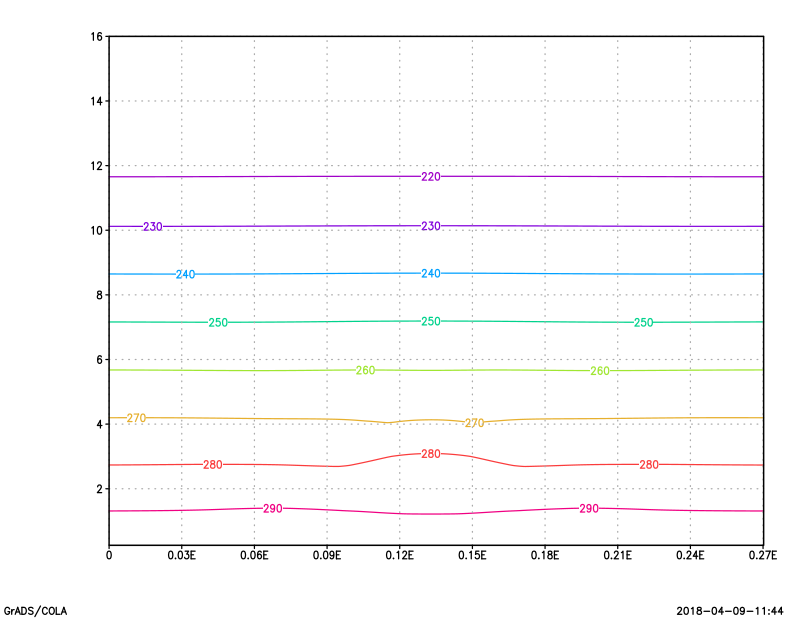
\includegraphics[width=.7\linewidth]{temperatura/Figuratk_tiempo_2.png}
  \caption{}
  \label{(a)}
\end{subfigure}%
\hskip -8ex  
\begin{subfigure}{.50\textwidth}
  \centering
  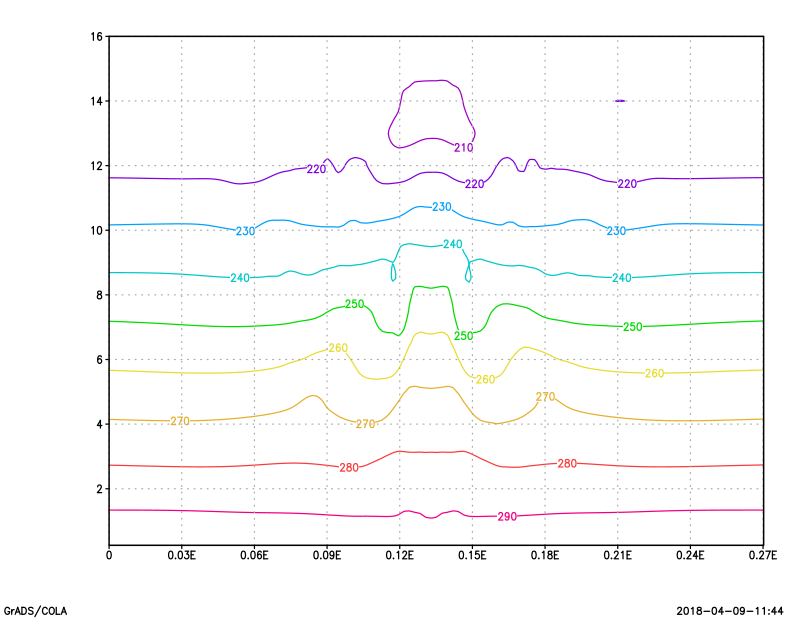
\includegraphics[width=.7\linewidth]{temperatura/Figuratk_tiempo_4}
  \caption{}
  \label{(b)}
\end{subfigure}
\hskip -8ex
\begin{subfigure}{.50\textwidth}
  \centering
  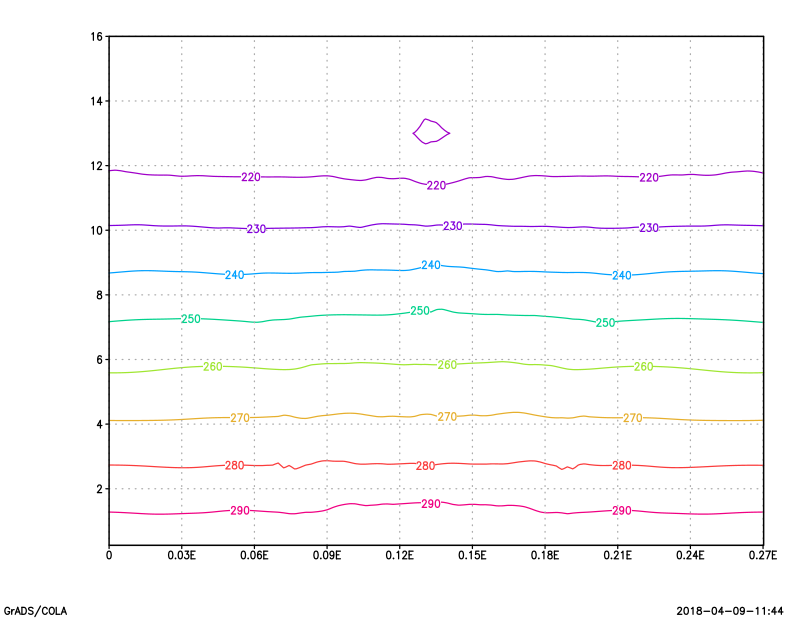
\includegraphics[width=.7\linewidth]{temperatura/Figuratk_tiempo_7}
  \caption{}
  \label{(c)}
\end{subfigure}
\hskip -8ex
\begin{subfigure}{.50\textwidth}
 \centering
  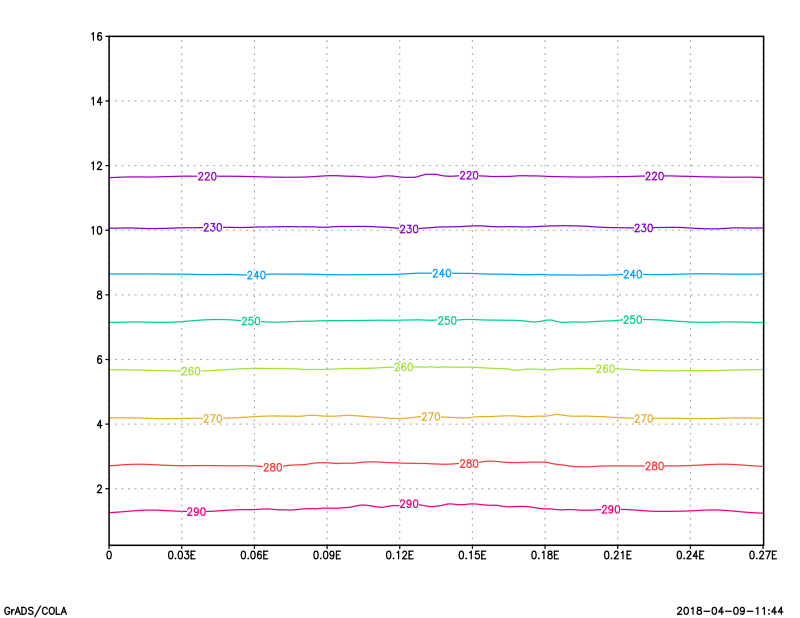
\includegraphics[width=.7\linewidth]{temperatura/Figuratk_tiempo_9}
  \caption{}
  \label{(d)}
\end{subfigure}%
\caption{\setstretch{1.0} Corte vertical de temperatura en Kelvin a) a los 10 minutos, b) 30 minutos, c) 60 minutos y d) 80 minutos de comenzada la simulación}
\label{Figura 3}
\end{figure}

\text{}\\ En la posición donde se encuentra la burbuja cálida, a los 10 minutos de comenzada la simulación se puede apreciar una perturbación de la temperatura en el segundo nivel en la vertical, más específicamente en la isolinea de 280 K. Esto indica la presencia de la burbuja de aire cálido que se pretendió simular. A los 30 minutos se puede ver cómo las perturbaciones se extendieron por todo el corte vertical, generando temperaturas más cálidas respecto del entorno por los 0.135E, mientras que alrededor de este valor, en 0.12E y 0.15E, se pueden apreciar temperaturas más frías que en el entorno. A los 60 minutos las perturbaciones de temperatura disminuyen, es decir que las temperaturas de la burbuja de aire cálido se asemejan a las del entorno, mostrando que la burbuja de aire cálido comienza a decaer. Finalmente, a los 80 minutos se puede observar que la temperatura es similar a la temperatura media en todos los niveles, no hay grandes perturbaciones.
\newpage

%% Imagen titae %%
\textbf{TEMPERATURA POTENCIAL EQUIVALENTE}

\begin{figure}[h!]
\centering
\begin{subfigure}{.50\textwidth}
 \centering
  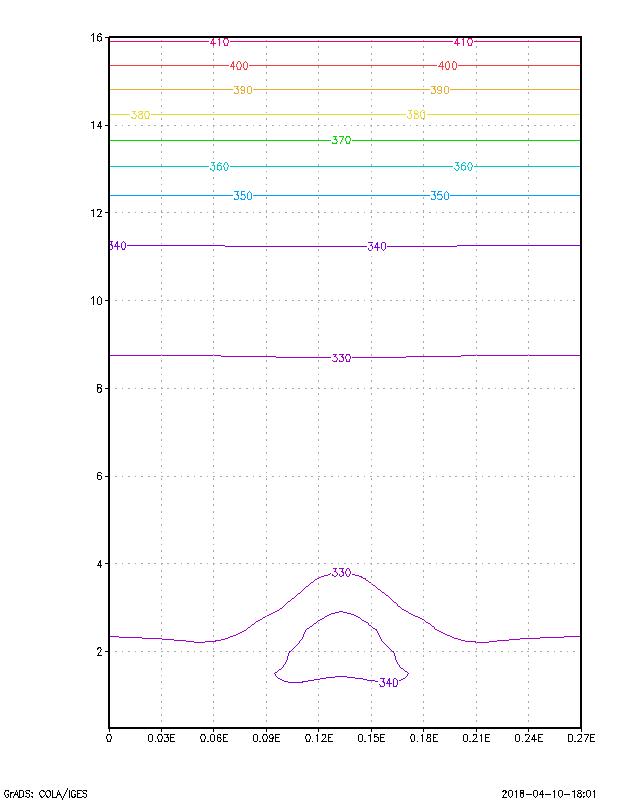
\includegraphics[width=.7\linewidth]{titae/Figura_titae_tiempo_2.png}
  \caption{}
  \label{(a)}
\end{subfigure}%
\hskip -8ex  
\begin{subfigure}{.50\textwidth}
  \centering
  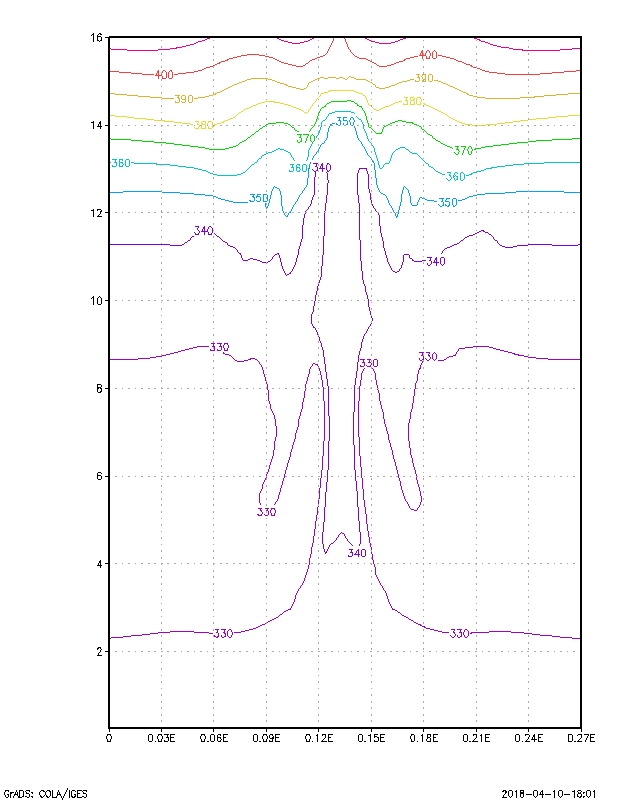
\includegraphics[width=.7\linewidth]{titae/Figura_titae_tiempo_4.png}
  \caption{}
  \label{(b)}
\end{subfigure}
\hskip -8ex
\begin{subfigure}{.50\textwidth}
  \centering
  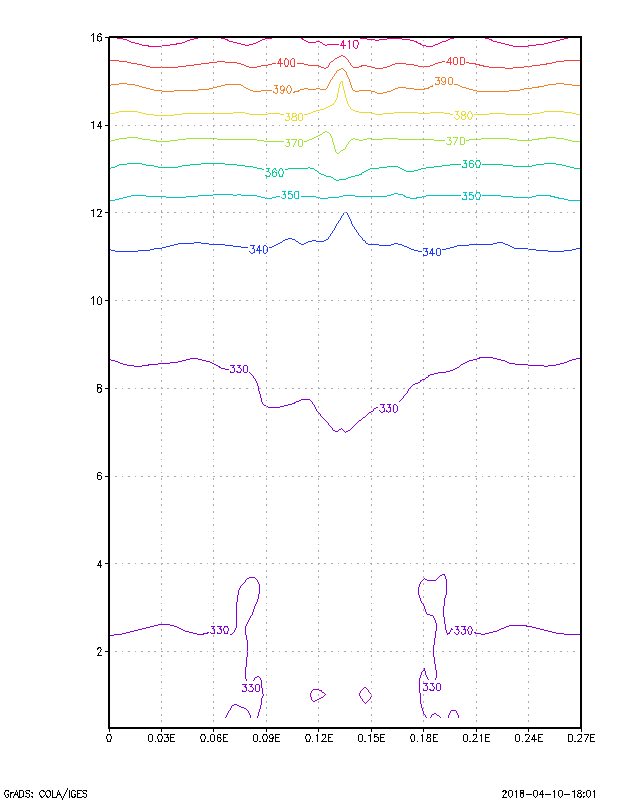
\includegraphics[width=.7\linewidth]{titae/Figura_titae_tiempo_7.png}
  \caption{}
  \label{(c)}
\end{subfigure}
\hskip -8ex
\begin{subfigure}{.50\textwidth}
 \centering
  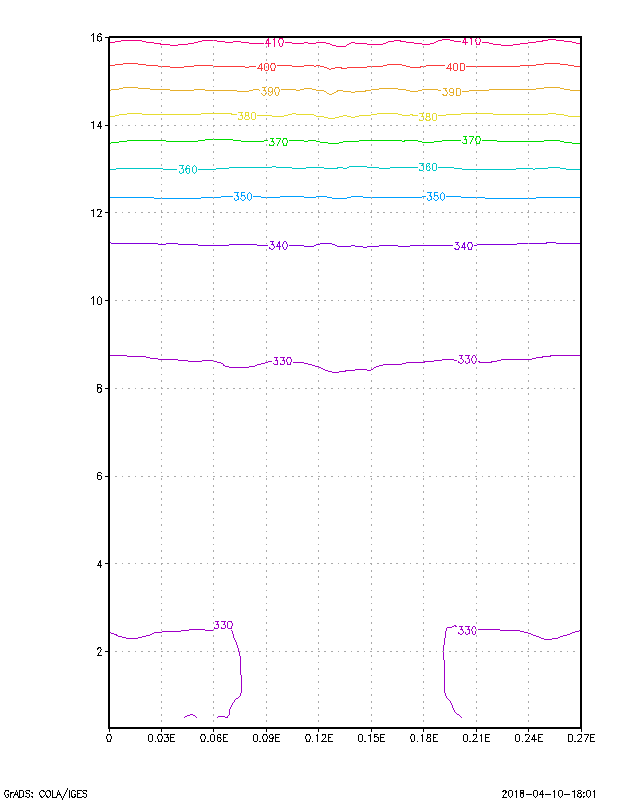
\includegraphics[width=.7\linewidth]{titae/Figura_titae_tiempo_9.png}
  \caption{}
  \label{(d)}
\end{subfigure}%
\caption{\setstretch{1.0} Corte vertical de temperatura equivalente en Kelvin a) a los 10 minutos, b) 30 minutos, c) 60 minutos y d) 80 minutos de comenzada la simulación}
\label{Figura 3}
\end{figure}


\text{}\\  La temperatura potencial equivalente \textTheta\textsubscript{e} es la temperatura que alcanzaría una parcela si luego de ser sometida a un proceso adiabático saturado reversible perdiese todo el contenido de vapor de agua. Utilizando esta variable se puede estudiar cómo asciende la burbuja de aire durante el proceso de convección, y cómo afecta a la distribución de la temperatura en la vertical sin tener en cuenta los efectos que pueden producir la presencia de humedad. \\
A los 10 minutos de comenzada la simulación (figura 2a) se observa una burbuja cálida incipiente: en superficie encontramos contornos de 340 K que perturban el campo de temperaturas. A los 30 minutos (figura 2b) se puede ver cómo la burbuja inicia de 340 K se expandió en la vertical y ascendió a mayores alturas y logra perturbar el perfil vertical de temperaturas en altura. A los 60 minutos (figura 2c) el campo de temperaturas comienza a estabilizarse nuevamente: ya no se observa una "mezcla" de temperaturas, sino que el campo tiende a volverse estratificado, con temperaturas más altas arriba y más bajas en niveles más cerca del suelo. Finalmente, a los 90 minutos (figura 2d) continua este proceso de estratificación, disminuyendo las perturbaciones de la burbuja de aire cálido sobre el campo de \textTheta\textsubscript{e}.


\textbf{VELOCIDAD VERTICAL}
\begin{figure}[h!]
\centering
\begin{subfigure}
{.50\textwidth}
 \centering
  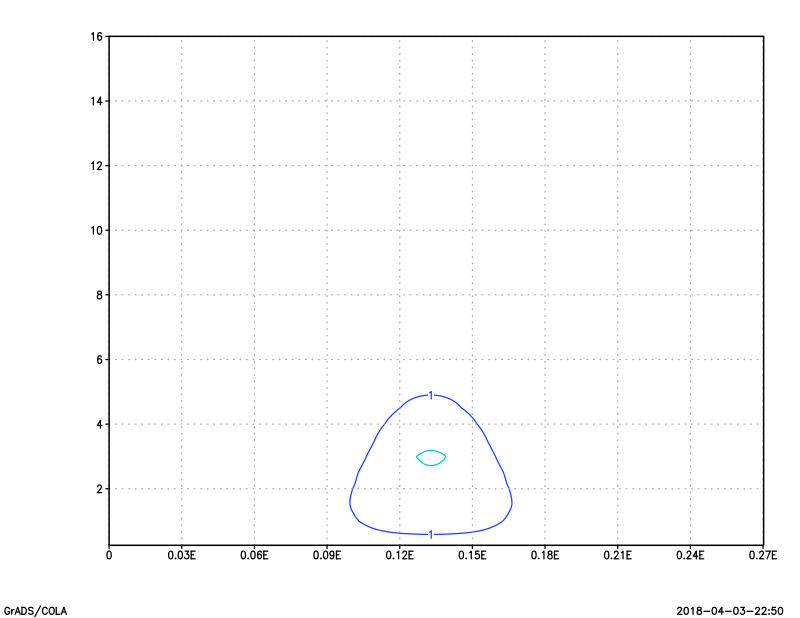
\includegraphics[width=.7\linewidth]{W/Figura_W_tiempo_2.png}
  \caption{}
  \label{(a)}
\end{subfigure}%
\hskip -8ex  
\begin{subfigure}{.50\textwidth}
  \centering
  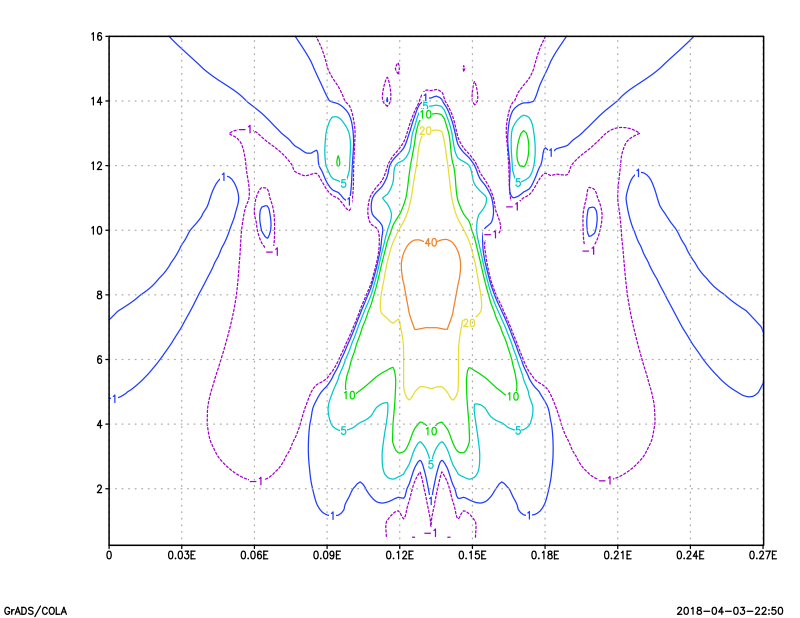
\includegraphics[width=.7\linewidth]{W/Figura_W_tiempo_4}
  \caption{}
  \label{(b)}
\end{subfigure}
\hskip -8ex
\begin{subfigure}{.50\textwidth}
  \centering
  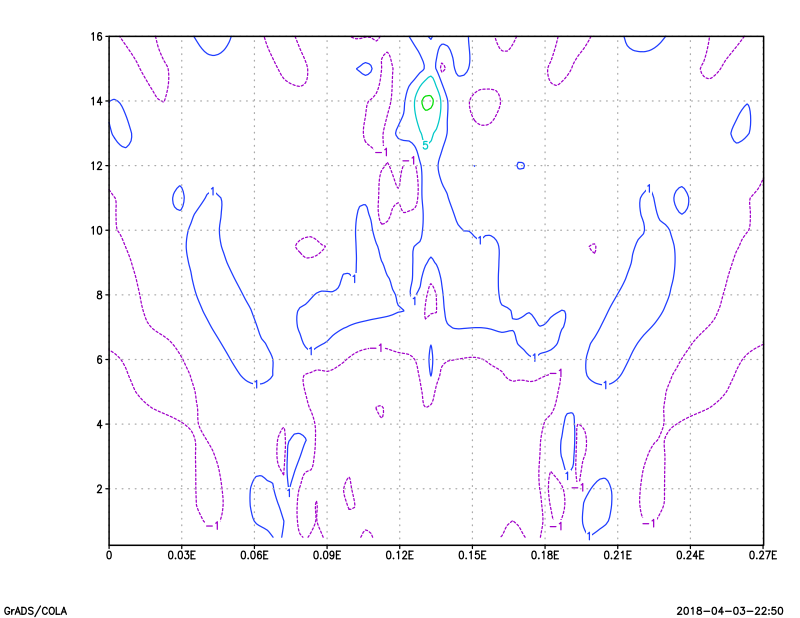
\includegraphics[width=.7\linewidth]{W/Figura_W_tiempo_7}
  \caption{}
  \label{(c)}
\end{subfigure}
\hskip -8ex
\begin{subfigure}{.50\textwidth}
 \centering
  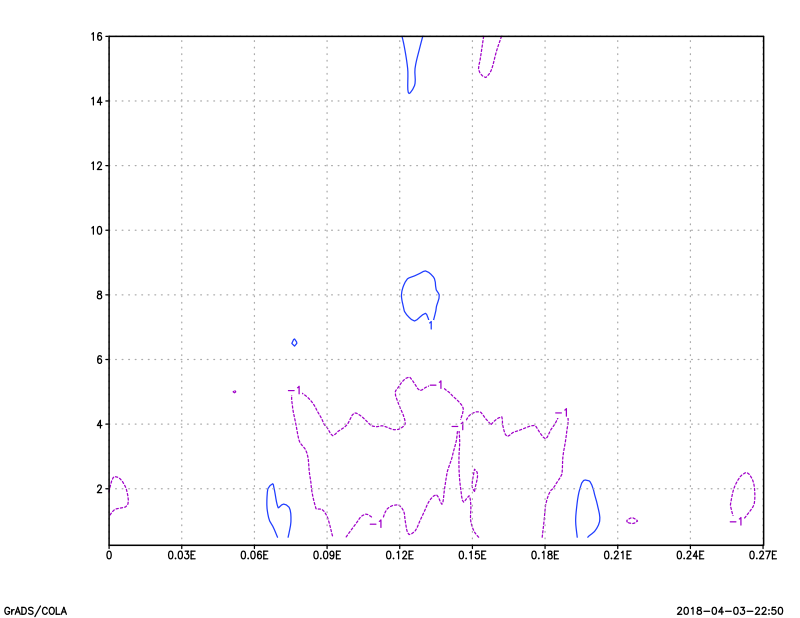
\includegraphics[width=.7\linewidth]{W/Figura_W_tiempo_9}
  \caption{}
  \label{(d)}
\end{subfigure}%
\caption{\setstretch{1.0} Corte vertical de W en m/seg a) a los 10 minutos, b) 30 minutos, c) 60 minutos y d) 80 minutos de comenzada la simulación}
\label{Figura 3}
\end{figure}
\text{}\\ A los 10 minutos de comenzada la simulación, la velocidad vertical (W) posee valores bajos o nulos. Luego, a los 30 minutos donde ya pueden comenzar a observarse los efectos de la convección, los valores de la velocidad vertical se vuelven mayores llegando hasta un máximo de 40 m/seg en el centro de la burbuja cálida. Por otro lado, a los lados de la posición de la burbuja cálida, se observan velocidades negativas, asociadas a movimientos descendentes. Sin embargo, los valores de estas velocidades son pequeños. \\ A los 60 minutos continua la configuración descrita previamente: valores positivos que indican ascensos sobre las regiones centrales, aproximadamente por la zona de la burbuja de aire cálido y valores negativos que indican descensos por los extremos de la burbuja. Sin embargo, los valores de los ascensos poseen módulo menor al tiempo previamente analizado: el máximo que se puede observar en la Figura 3c) es de 20 m/seg. Esto indica que la convección se desacelera como consecuencia de la mezcla del aire de la burbuja de aire cálido con el aire del entorno.\\ Finalmente a los 90 minutos las velocidades verticales se vuelven casi nulas, tomando valores ascendentes y descendentes pero de módulo de aproximadamente 1 m/seg. 

\textbf{VELOCIDAD HORIZONTAL: U}
\begin{figure}[h!]
\centering
\begin{subfigure}
{.50\textwidth}
 \centering
  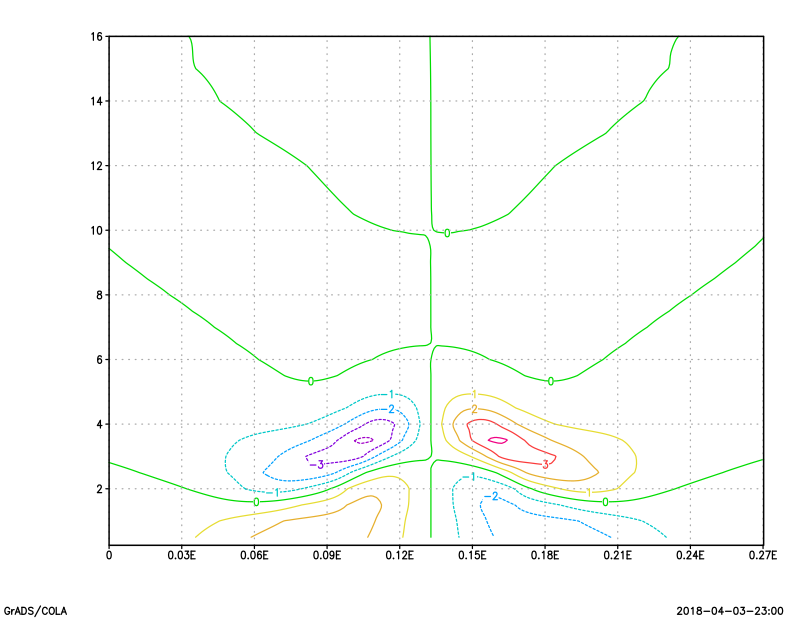
\includegraphics[width=.7\linewidth]{U/Figura_umet_tiempo_2.png}
  \caption{}
  \label{(a)}
\end{subfigure}%
\hskip -8ex  
\begin{subfigure}{.50\textwidth}
  \centering
  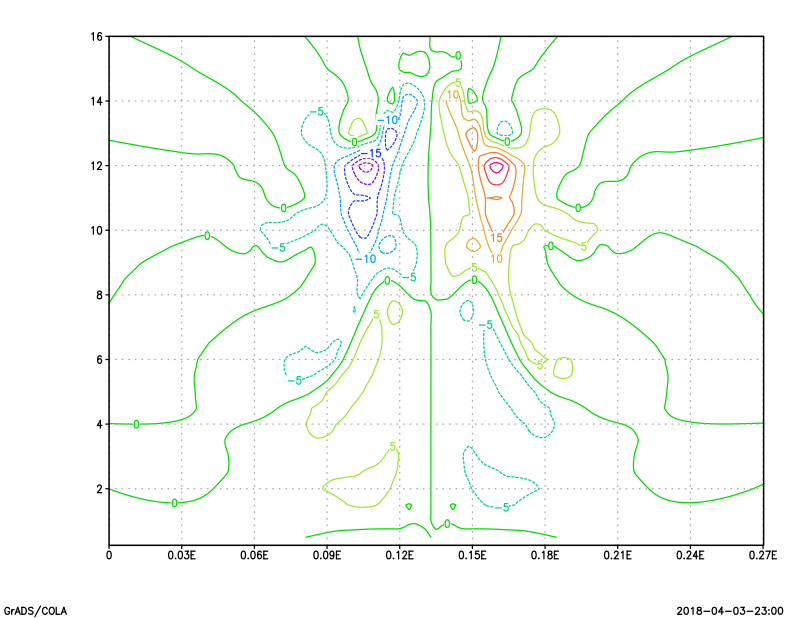
\includegraphics[width=.7\linewidth]{U/Figura_umet_tiempo_4.png}
  \caption{}
  \label{(b)}
\end{subfigure}
\hskip -8ex
\begin{subfigure}{.50\textwidth}
  \centering
  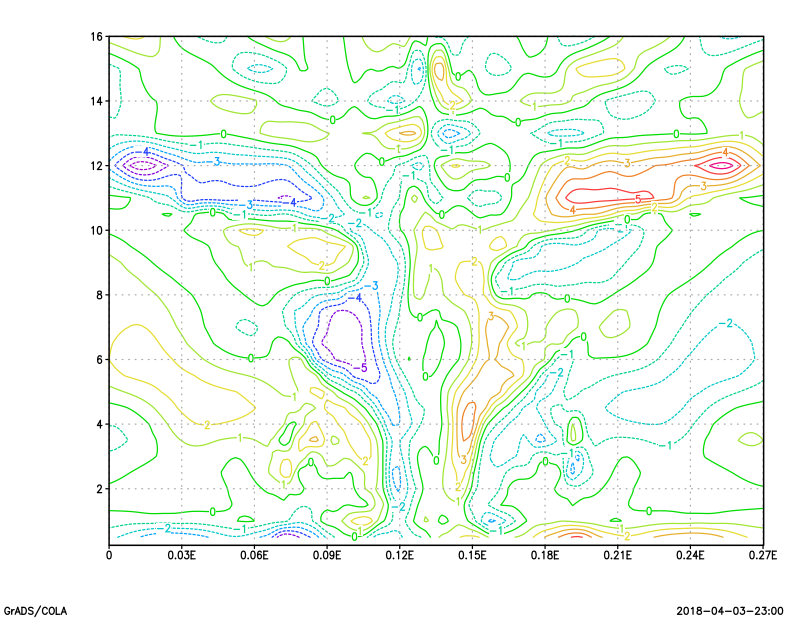
\includegraphics[width=.7\linewidth]{U/Figura_umet_tiempo_7.png}
  \caption{}
  \label{(c)}
\end{subfigure}
\hskip -8ex
\begin{subfigure}{.50\textwidth}
 \centering
  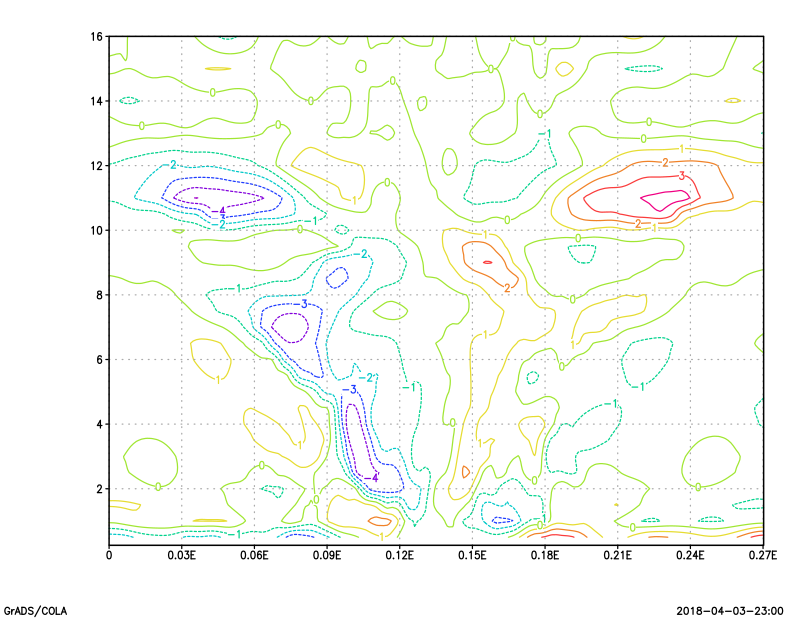
\includegraphics[width=.7\linewidth]{U/Figura_umet_tiempo_9.png}
  \caption{}
  \label{(d)}
\end{subfigure}%
\caption{\setstretch{1.0} Corte vertical de U en m/seg a) a los 10 minutos, b) 30 minutos, c) 60 minutos y d) 80 minutos de comenzada la simulación}
\label{Figura 3}
\end{figure}
\text{}\\Observando la figura 4a, a los 10 minutos de comenzada la simulación, a la derecha e izquierda de la posición de la burbuja de aire cálido se observan valores opuestos de velocidad horizontal. En la superficie (hasta el nivel 3 de altura), a la derecha de la zona donde se encuentra la burbuja de aire cálido, se encuentran valores negativos de velocidad horizontal en la dirección de x, mientras que a la izquierda, valores positivos. Esto quiere decir que en superficie el aire se dirige hacia la posición de la burbuja de aire cálido. En cambio hasta el nivel 6 de altura la configuración de velocidades es la opuesta: a la izquierda valores negativos y a la derecha valores positivos de velocidad U, es decir que a esta altura el aire tiende a alejarse de la posición donde se encuentra la burbuja de aire. \\ A los 30 minutos de comenzada la simulación (figura 4b) el caso es similar a lo observado en el tiempo anterior: en superficie vientos que se dirigen hacia la posición de la burbuja de aire cálido, y en altura vientos que parten desde ella. Sin embargo, en este tiempo la magnitud de los vientos es diferente dependiendo de la altura en la que s encuentren, en altura alcanzan velocidades máximas de 20 m/seg mientras que en superficie las velocidades máximas son de 5 m/seg. \\ A los 60 minutos (figura 4c) el campo de velocidades de U se encuentra más desordenado, es decir que a las distintas alturas ya no se distinguen tan claramente zonas horizontales donde el viento se dirija desde o hacia la burbuja de aire cálido, sino que estas zonas se alternan. Sin embargo en este tiempo, este comportamiento es más visible en las zonas bajas que en las zonas altas y en las zonas más alejadas de la burbuja de aire, ya que por niveles medios a un lado y otro de la burbuja de aire se aprecian sentidos opuestos de desplazamiento del viento horizontal U. Otro aspecto a destacar es que en este tiempo, la magnitud de los vientos disminuyó respecto de la magnitud del tiempo anterior aunque los valores del viento en niveles superiores continúa siendo mayor en altura.\\ Finalmente, a los 90 minutos (figura 4d) el campo de vientos U se observa aún más desordenado, aunque en altura predominan vientos que se alejan de la burbuja de aire: hacia el Este a la derecha de la burbuja y hacia el Oeste a la izquierda de la misma; y en superficie vientos que se dirigen hacia la posición original de la burbuja de aire. 

\textbf{VELOCIDAD HORIZONTAL: V}
\begin{figure}[h!]
\centering
\begin{subfigure}
{.50\textwidth}
 \centering
  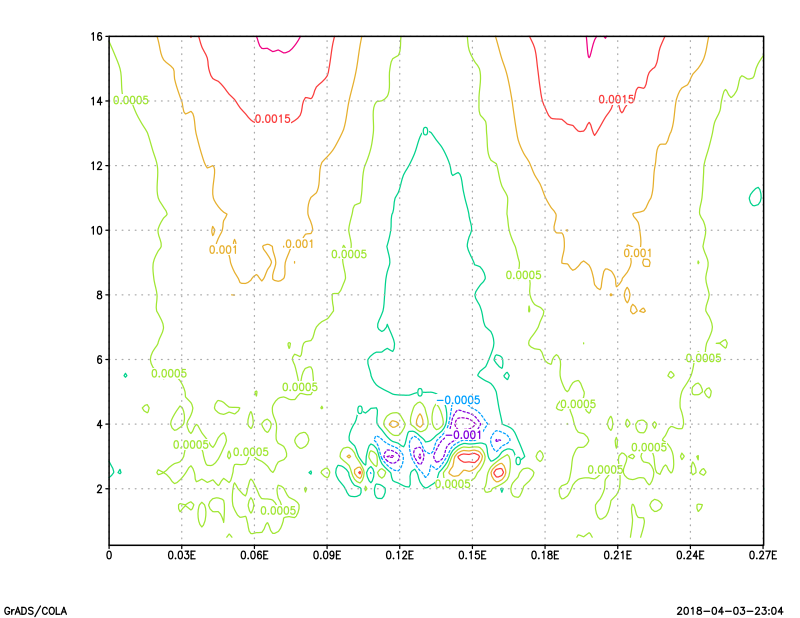
\includegraphics[width=.7\linewidth]{V/Figura_v_tiempo_2.png}
  \caption{}
  \label{(a)}
\end{subfigure}%
\hskip -8ex  
\begin{subfigure}{.50\textwidth}
  \centering
  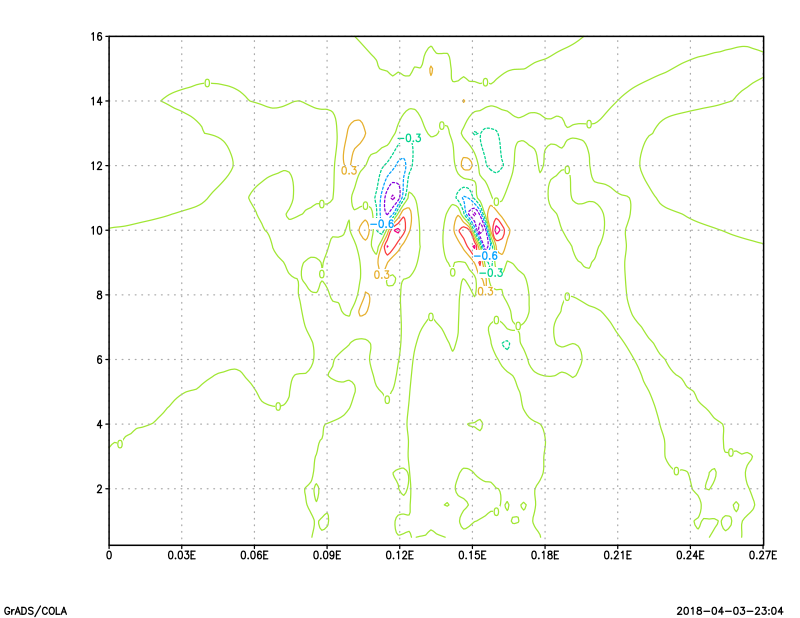
\includegraphics[width=.7\linewidth]{V/Figura_v_tiempo_4.png}
  \caption{}
  \label{(b)}
\end{subfigure}
\hskip -8ex
\begin{subfigure}{.50\textwidth}
  \centering
  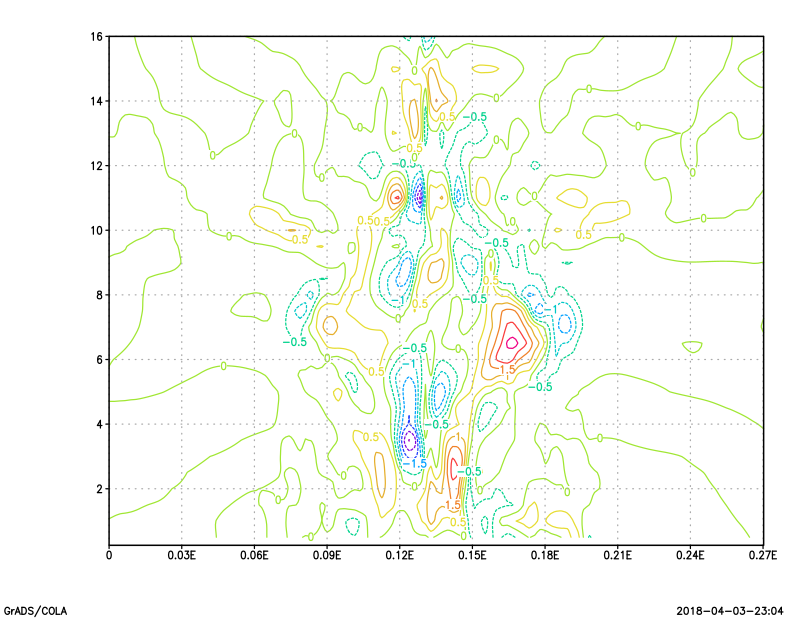
\includegraphics[width=.7\linewidth]{V/Figura_v_tiempo_7.png}
  \caption{}
  \label{(c)}
\end{subfigure}
\hskip -8ex
\begin{subfigure}{.50\textwidth}
 \centering
  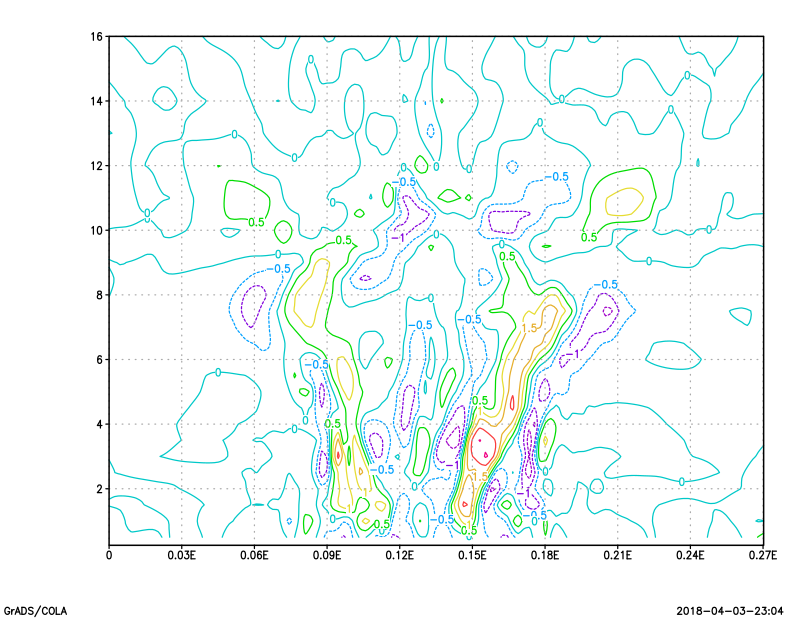
\includegraphics[width=.7\linewidth]{V/Figura_v_tiempo_9.png}
  \caption{}
  \label{(d)}
\end{subfigure}%
\caption{\setstretch{1.0} Corte vertical de V en m/s a) a los 10 minutos, b) 30 minutos, c) 60 minutos y d) 80 minutos de comenzada la simulación}
\label{Figura 3}
\end{figure}

\text{}\\A los 10 minutos del comienzo de la simulación (figura 5a) se observa que en niveles altos y en niveles bajos alejados del punto donde se encuentra la burbuja de aire cálido el viento es Sur (valores positivos). Sin embargo, donde se encuentra la burbuja de aire cálido se observan valores de viento V tanto positivos como negativos, es decir con sentidos opuestos. En cambio a los 30 minutos (figura 5b) el campo de velocidades V se vuelve más ordenado, mostrando vientos distintos de cero (del Norte y Sur) en niveles superiores. En este tiempo la magnitud de los vientos comienza a aumentar. Luego, a los 60 minutos el campo comienza a desorganizarse nuevamente y la magnitud de los vientos continua aumentando, mostrando valores significativos de viento Norte y Sur cerca de la posición de la burbuja de aire cálido y sobre todo en altura. Finalmente, a los 90 minutos (figura 5d) los mayores valores de viento V se desplazaron hacia los niveles más bajos. \\ Algo para destacar es que la magnitud del viento V es mucho menor comparada con la magnitud del viento U, siendo el valor máximo observado para el primero de 1.5 m/seg, mientras que para el segundo es de 15 m/seg. Es decir que para el proceso de convección será más relevante el efecto producido sobre el viento U.

\textbf{CANTIDAD TOTAL DE CONDENSADO}
\begin{figure}[h!]
\centering
\begin{subfigure}
{.50\textwidth}
 \centering
  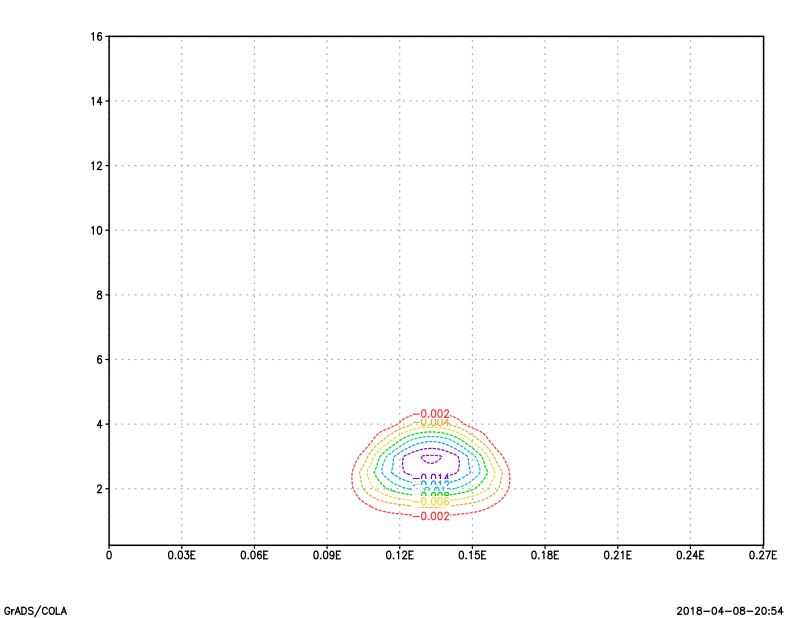
\includegraphics[width=.7\linewidth]{QTOT/Figura_QC_tiempo_2.png}
  \caption{}
  \label{(a)}
\end{subfigure}%
\hskip -8ex  
\begin{subfigure}{.50\textwidth}
  \centering
  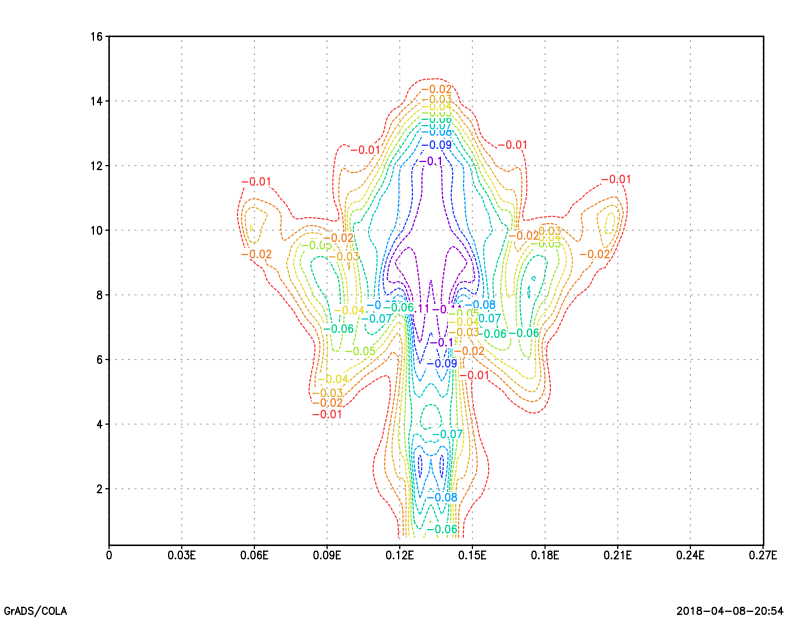
\includegraphics[width=.7\linewidth]{QTOT/Figura_QC_tiempo_4.png}
  \caption{}
  \label{(b)}
\end{subfigure}
\hskip -8ex
\begin{subfigure}{.50\textwidth}
  \centering
  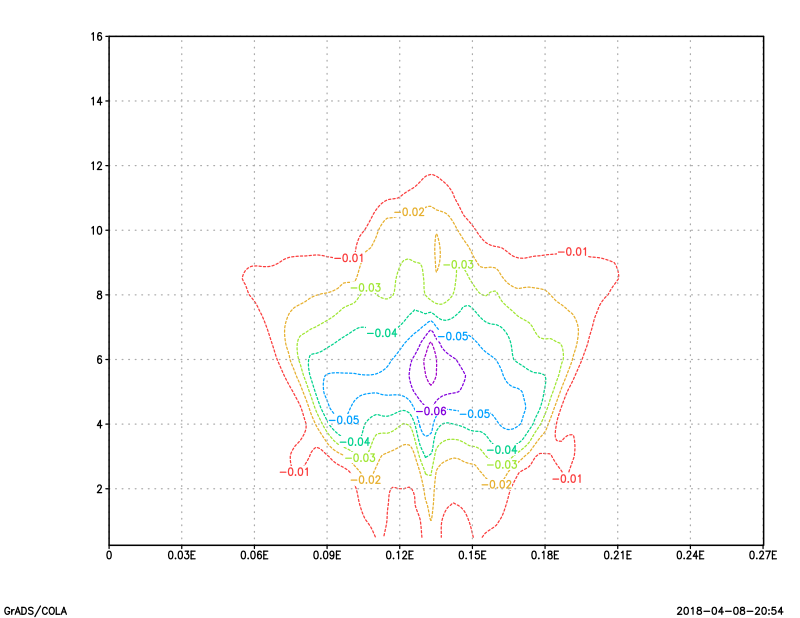
\includegraphics[width=.7\linewidth]{QTOT/Figura_QC_tiempo_7.png}
  \caption{}
  \label{(c)}
\end{subfigure}
\hskip -8ex
\begin{subfigure}{.50\textwidth}
 \centering
  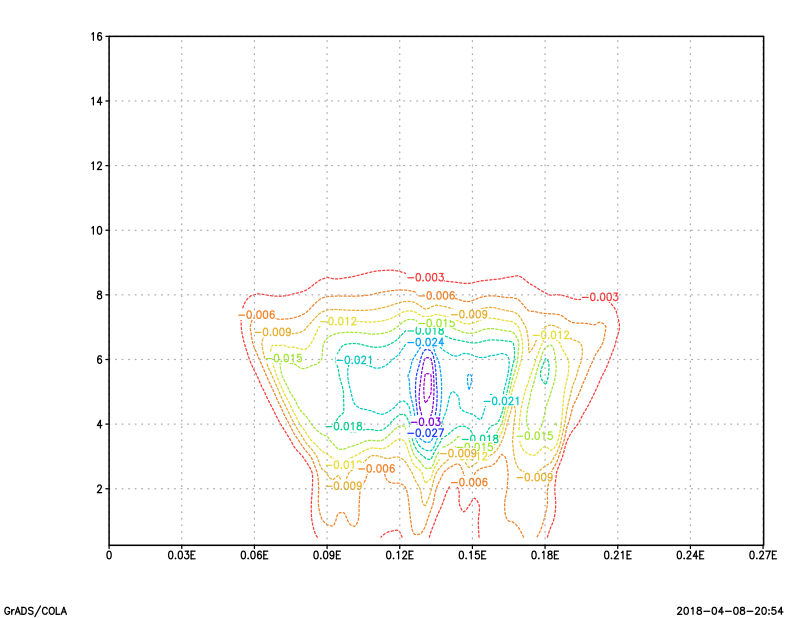
\includegraphics[width=.7\linewidth]{QTOT/Figura_QC_tiempo_9.png}
  \caption{}
  \label{(d)}
\end{subfigure}%
\caption{\setstretch{1.0} Corte vertical de cantidad total de condensado en kg/kg a) a los 10 minutos, b) 30 minutos, c) 60 minutos y d) 80 minutos de comenzada la simulación}
\label{Figura 3}
\end{figure}
\text{}\\En primer lugar es importante aclarar que los valores de condensado total graficados en la figura 6 son negativos ya que corresponden al aporte del condensado al empuje, que como se verá más adelante afecta negativamente al empuje. \\ A los 10 minutos del comienzo de la simulación (figura 6a) los niveles más cercanos al suelo comienzan a presentar condensado como consecuencia de los ascensos de aire que se producen desde la superficie. A los 30 minutos (figura 6b) la presencia de condensado se extiende sobre niveles superiores, donde también la magnitud del condensado aumenta. No sólo eso, sino que también el condensado comienza a expandirse en la horizontal, sobre todo en niveles superiores. A los 60 minutos (figura 6c) se puede observar que la magnitud del condensado disminuyó considerablemente, como así también la altura máxima hasta la que se extiende el condensado; en cambio, en la horizontal la distribución del condensado no disminuyó su extensión. Finalmente, a los 90 minutos (figura 6d) la magnitud del condensado disminuyó nuevamente, alcanzando valores máximos de 0.03, como así también su extensión en la vertical.
\newpage{}
\textbf{CALOR DIABÁTICO}
\begin{figure}[h!]
\centering
\begin{subfigure}
{.50\textwidth}
 \centering
  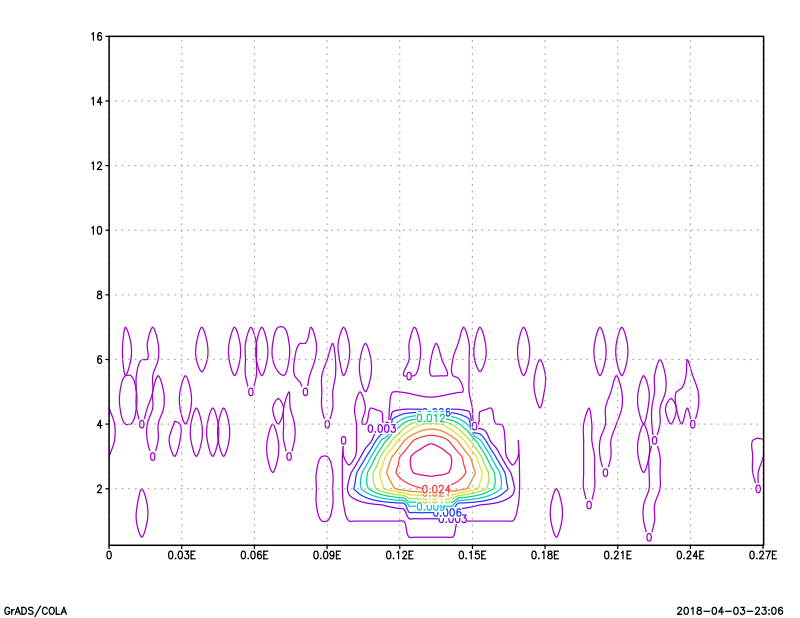
\includegraphics[width=.7\linewidth]{CDIAB/Figura_diabatico_tiempo_2.png}
  \caption{}
  \label{(a)}
\end{subfigure}%
\hskip -8ex  
\begin{subfigure}{.50\textwidth}
  \centering
  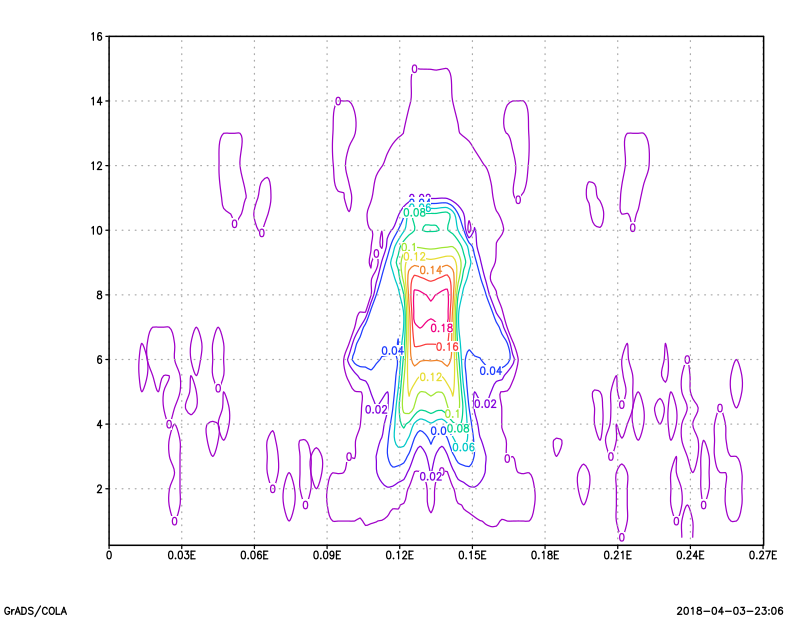
\includegraphics[width=.7\linewidth]{CDIAB/Figura_diabatico_tiempo_4.png}
  \caption{}
  \label{(b)}
\end{subfigure}
\hskip -8ex
\begin{subfigure}{.50\textwidth}
  \centering
  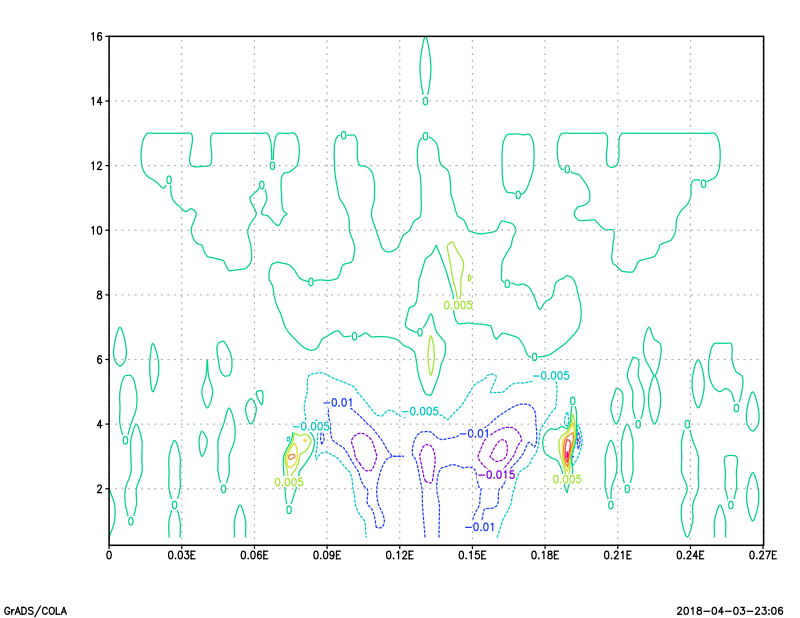
\includegraphics[width=.7\linewidth]{CDIAB/Figura_diabatico_tiempo_7.png}
  \caption{}
  \label{(c)}
\end{subfigure}
\hskip -8ex
\begin{subfigure}{.50\textwidth}
 \centering
  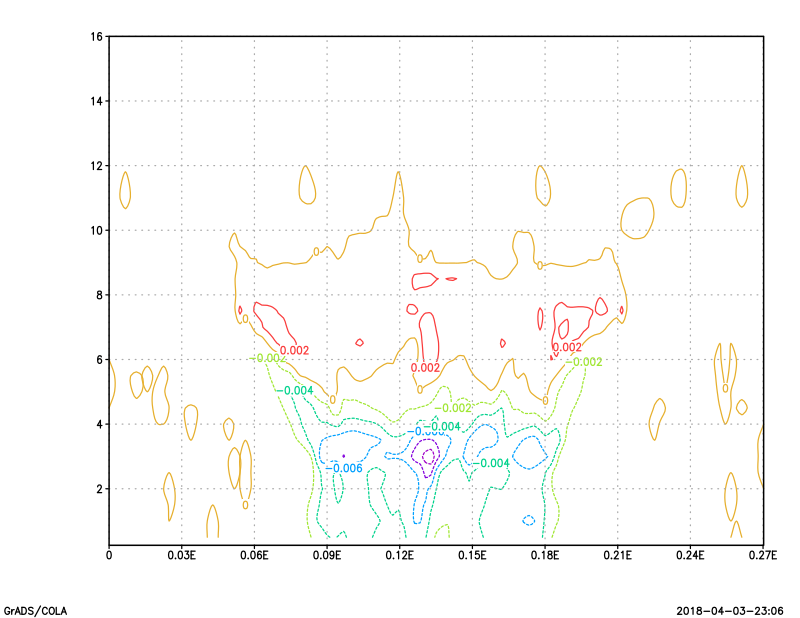
\includegraphics[width=.7\linewidth]{CDIAB/Figura_diabatico_tiempo_9.png}
  \caption{}
  \label{(d)}
\end{subfigure}%
\caption{\setstretch{1.0} Corte vertical de Calor diabático en K/seg a) a los 10 minutos, b) 30 minutos, c) 60 minutos y d) 80 minutos de comenzada la simulación}
\label{Figura 3}
\end{figure}
\text{} \\Calor diabático: Al comienzo de la convección (10 min) se ven valores positivos de calor diabático debido a la emanación de calor latente por la condensación en el ascenso. Luego a los 30 min se ve un aumento del calor diabático, llegando a la máxima emisión de calor latente en niveles altos. Luego de esto, la nube precipita y genera enfriamiento en niveles bajos por la evaporación de las gotas de lluvia, por lo tanto se ven valores negativos de calor diabático. Y por último, a los 80 min, se ven valores positivos en niveles medios y negativos cerca de superficie (pileta fria). \\


%%%%%%%%%%%%%%%%%%%%%%%%%%%%%%%%%%%%%%%%%%%%%%%%%
\newpage{}
\textbf{b) Para  esos  mismos  tiempos  calcule:  la  aceleración  vertical,  el  empuje,  las 
perturbaciones   de   presión,   el   gradiente   vertical   de   perturbaciones   de 
presión, la perturbación de temperatura y la perturbación
de humedad
}


\textbf{ACELERACION VERTICAL}
\begin{figure}[h!]
\centering
\begin{subfigure}
{.50\textwidth}
 \centering
  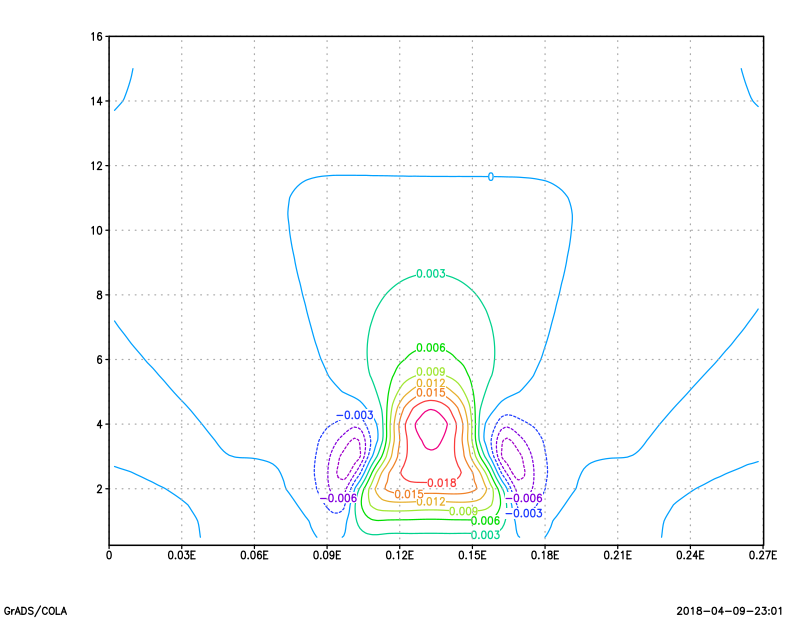
\includegraphics[width=.7\linewidth]{dwdt/DWDT_tiempo_2.png}
  \caption{}
  \label{(a)}
\end{subfigure}%
\hskip -8ex  
\begin{subfigure}{.50\textwidth}
  \centering
  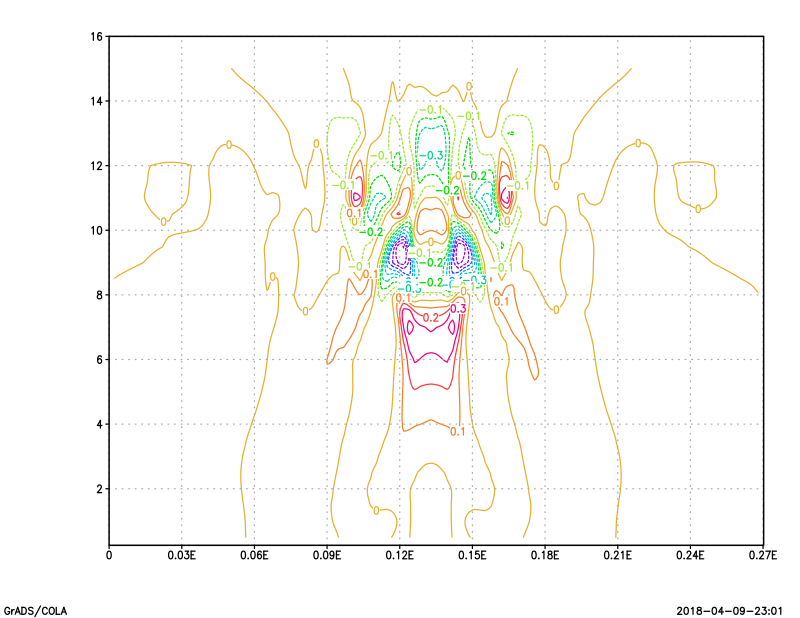
\includegraphics[width=.7\linewidth]{dwdt/DWDT_tiempo_4.png}
  \caption{}
  \label{(b)}
\end{subfigure}
\hskip -8ex
\begin{subfigure}{.50\textwidth}
  \centering
  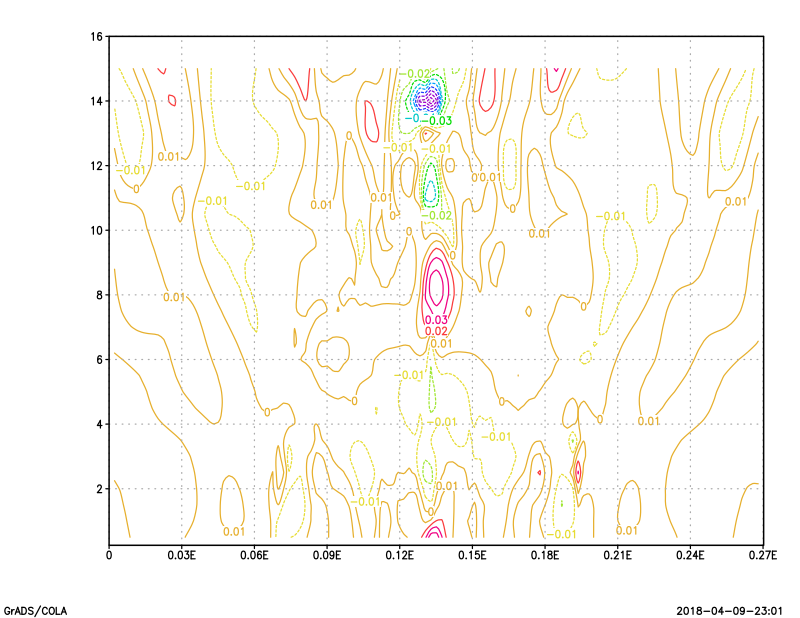
\includegraphics[width=.7\linewidth]{dwdt/DWDT_tiempo_7.png}
  \caption{}
  \label{(c)}
\end{subfigure}
\hskip -8ex
\begin{subfigure}{.50\textwidth}
 \centering
  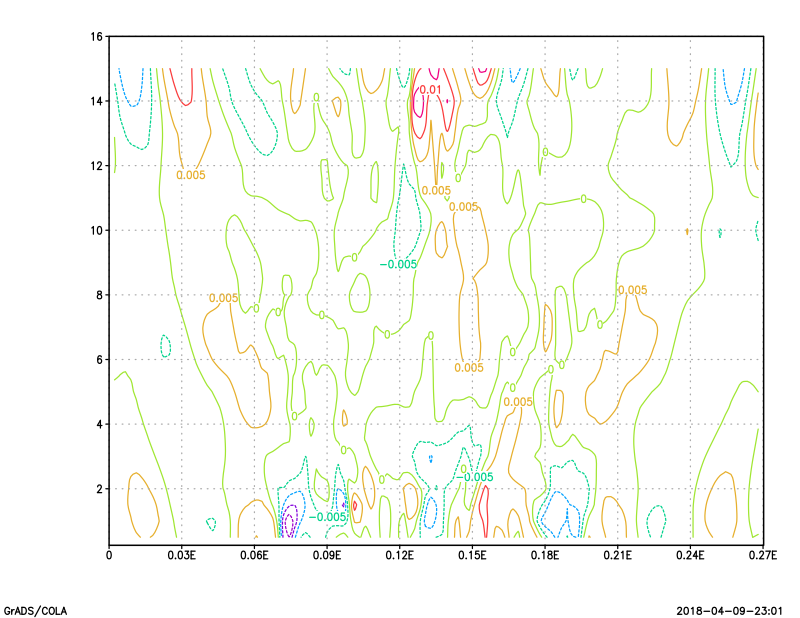
\includegraphics[width=.7\linewidth]{dwdt/DWDT_tiempo_9.png}
  \caption{}
  \label{(d)}
\end{subfigure}%
\caption{\setstretch{1.0} Corte vertical de aceleración vertical en m/seg² a) a los 10 minutos, b) 30 minutos, c) 60 minutos y d) 80 minutos de comenzada la simulación}
\label{Figura 3}
\end{figure}
\newpage{}

%%%%%%%%%%%%%%5
\textbf{Perturbaciones de presión}
\begin{figure}[h!]
\centering
\begin{subfigure}
{.50\textwidth}
 \centering
  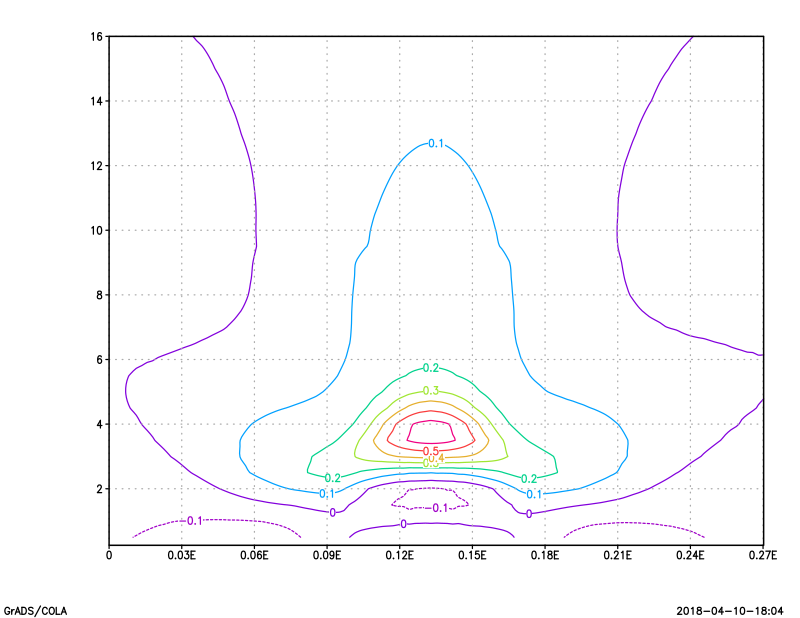
\includegraphics[width=.7\linewidth]{pprima/Figura_PPRIMA_tiempo_2.png}
  \caption{}
  \label{(a)}
\end{subfigure}%
\hskip -8ex  
\begin{subfigure}{.50\textwidth}
  \centering
  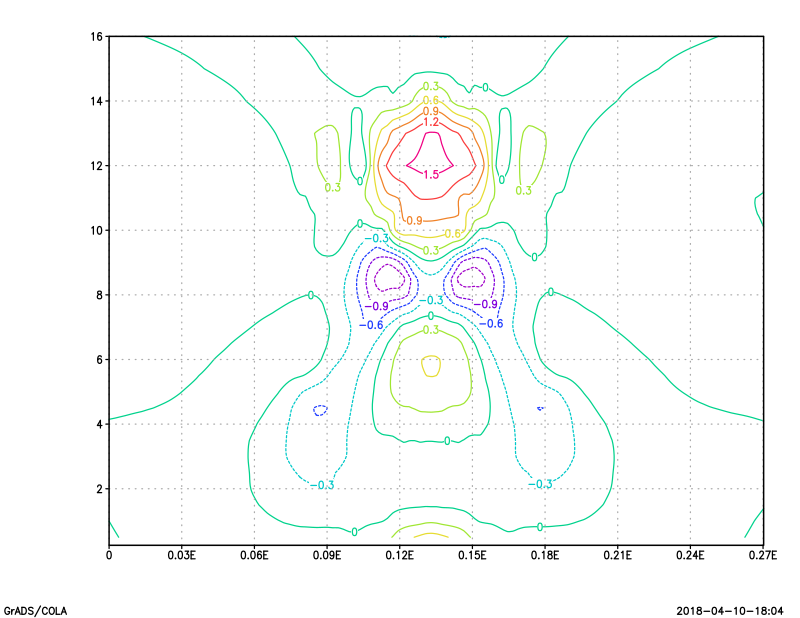
\includegraphics[width=.7\linewidth]{pprima/Figura_PPRIMA_tiempo_4.png}
  \caption{}
  \label{(b)}
\end{subfigure}
\hskip -8ex
\begin{subfigure}{.50\textwidth}
  \centering
  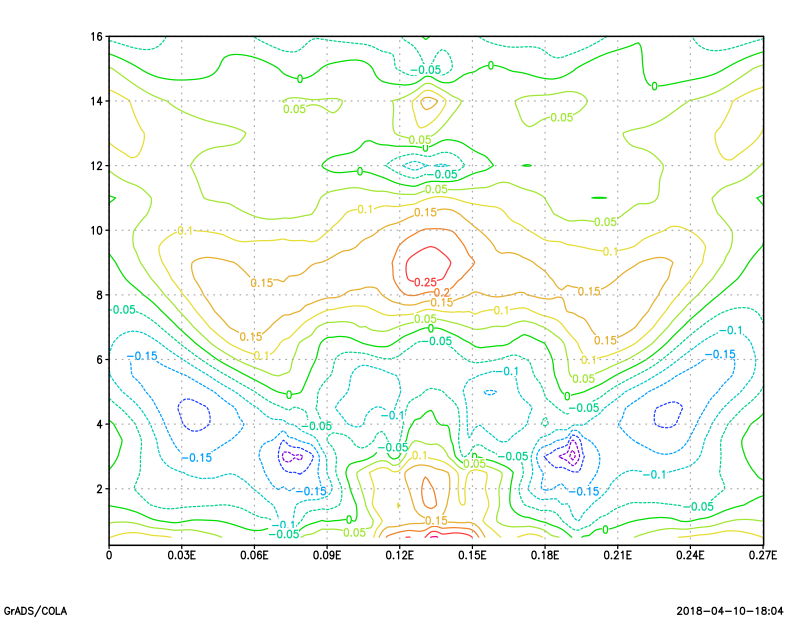
\includegraphics[width=.7\linewidth]{pprima/Figura_PPRIMA_tiempo_7.png}
  \caption{}
  \label{(c)}
\end{subfigure}
\hskip -8ex
\begin{subfigure}{.50\textwidth}
 \centering
  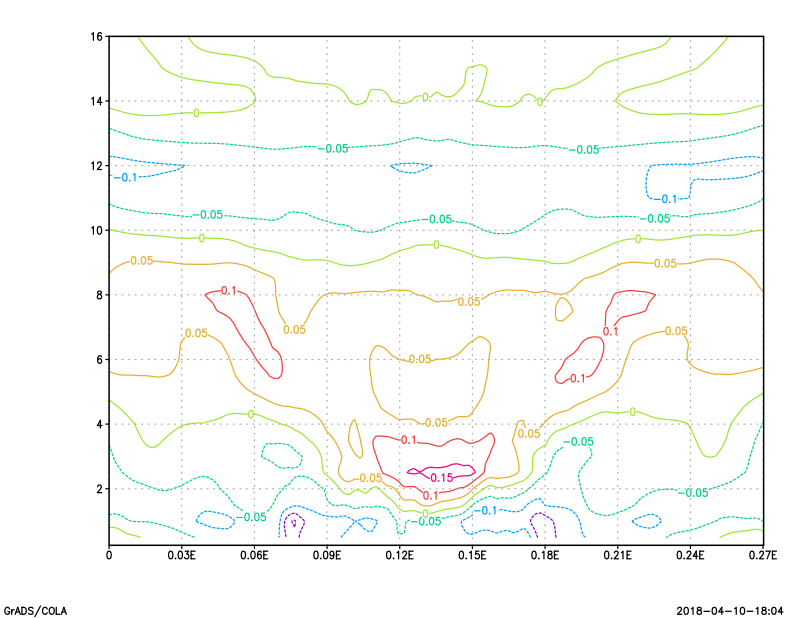
\includegraphics[width=.7\linewidth]{pprima/Figura_PPRIMA_tiempo_9.png}
  \caption{}
  \label{(d)}
\end{subfigure}%
\caption{\setstretch{1.0} Corte vertical de P' en hPa a) a los 10 minutos, b) 30 minutos, c) 60 minutos y d) 80 minutos de comenzada la simulación}
\label{Figura 3}
\end{figure}
\text{} \\ Al comienzo se observan perturbaciones de presión negativas en superficie, lo que genera convergencia, y positivas en alturas medias (Divergencia). Al considerar las perturbaciones como funciones armónicas, P' se vuelve inversamente proporcional a la variación de B con la altura. A los 30 min se desarrolla completamente la nube y vemos las máximas perturbaciones de presión en niveles altos debido al gradiente negativo del empuje en la vertical.Luego a los 60 min vemos una franja en alturas medias de perturbaciones de presión negativa y positiva en superficie (asociada a descensos (con lluvia). Por ultimo a los 90 min vemos perturbaciones positivas en gran parte de la troposfera, donde se dan las mayores subsidencias. \\

\newpage{}
\textbf{Variaciones de P' con la vertical}
\begin{figure}[h!]
\centering
\begin{subfigure}
{.50\textwidth}
 \centering
  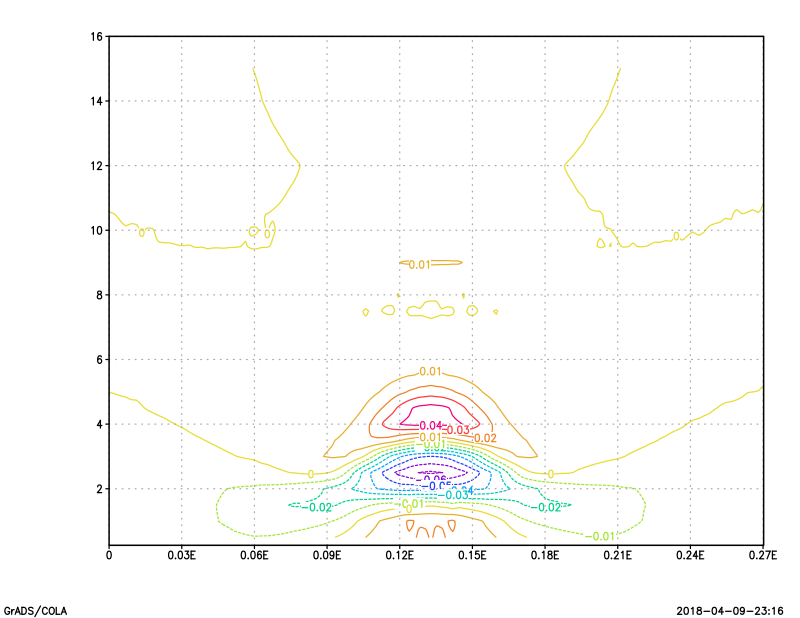
\includegraphics[width=.7\linewidth]{dPprimaDZ/DPPRIMADZ_tiempo_2.png}
  \caption{}
  \label{(a)}
\end{subfigure}%
\hskip -8ex  
\begin{subfigure}{.50\textwidth}
  \centering
  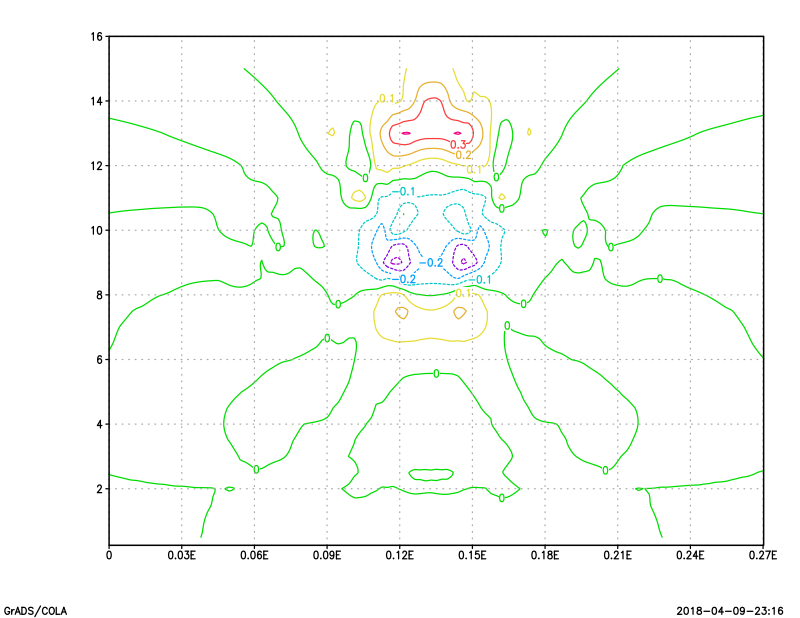
\includegraphics[width=.7\linewidth]{dPprimaDZ/DPPRIMADZ_tiempo_4.png}
  \caption{}
  \label{(b)}
\end{subfigure}
\hskip -8ex
\begin{subfigure}{.50\textwidth}
  \centering
  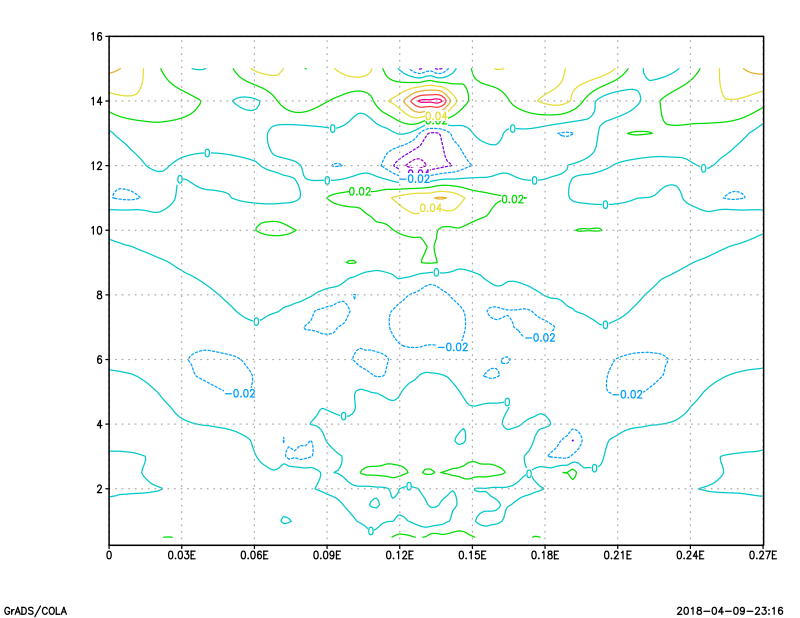
\includegraphics[width=.7\linewidth]{dPprimaDZ/DPPRIMADZ_tiempo_7.png}
  \caption{}
  \label{(c)}
\end{subfigure}
\hskip -8ex
\begin{subfigure}{.50\textwidth}
 \centering
  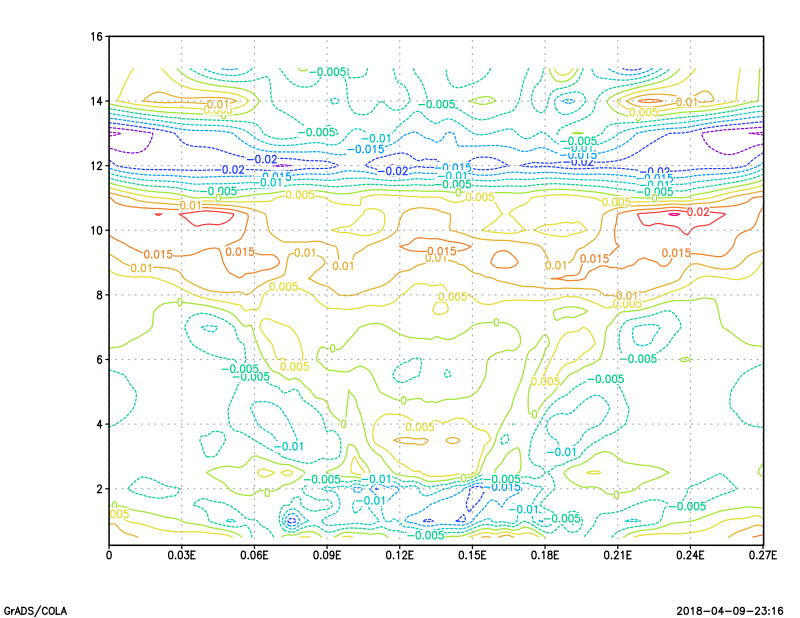
\includegraphics[width=.7\linewidth]{dPprimaDZ/DPPRIMADZ_tiempo_9.png}
  \caption{}
  \label{(d)}
\end{subfigure}%
\caption{\setstretch{1.0} Corte vertical de dP'/dz en hPa/km
a) a los 10 minutos, b) 30 minutos, c) 60 minutos y d) 80 minutos de comenzada la simulación}
\label{Figura 3}
\end{figure}
\text{} \\Es importante aclarar que las variaciones de p' con la altura están relacionadas a las aceleraciones verticales, donde tenemos maximos valores negativos de dp'/dz, tenemos máximos valores positivos de dw'/dt. A los 10 min se ven valores muy negativos cerca de superficie y máximos positivos por encima, esto nos da una idea de a que altura se encuentra el máximo w. El gradiente máximo de p' en altura esta relacionado con la variacion de esta variable desde el centro de la nube hasta el tope donde tenemos valores positivos de p'. A los 30 min siguen habiendo valores negativos de p' dentro de la nube, lo que nos indica velocidades de ascenso positivas que se mantienen. Luego precipita y a los 60 min ya no se ven claros estos gradientes que se dan dentro de la nube y por ultimo a los 80 min se ven valores positivos en niveles bajos y medios de la atmosfera lo que nos muestra una aceleración negativa de w, asociada a descenso con secamiento y enfriamiento. \\

%%%%%%%%%%%%%%%%%%%%%%%%%%%%%%%%%%%%%%%%%%%%%%%%%
\newpage{}
\newpage{}

\textbf{c) Identifique  el  intervalo  temporal  y  posición  espacial  donde  el  término 
asociado a las perturbaciones de presión aportan positiva y negativamente a 
las aceleraciones verticales.
}
\text{}\\ Subsidencia en los costados. Tiempo 40: ascensos más débiles por P'. Aportes negativos abajo (asociadas al entrainment) y positivos arriba (baja presión arriba). En tiempos siguientes es lo contrario. Aporte de P' desde los 30 min.\\
T': T'<0 en el tope de la nube. Costados celestes: enfriamiento por evaporación de los costados de la nube. Mayor cantidad de aporte (en módulo y temporal) de T' que de P'. \\

Aporte de qh: aporte negativo al empuje. La masa de los hidrometeoros frenan los ascensos en la nube (opuesto al aporte de la temperatura). \\

dp'/dz: 



%%%%%%%%%%%%%%%%%%%%%%%%%%%%%%%%%%%%%%%%%%%%%%%%%
\textbf{d) Identifique  el  intervalo  temporal  y  posición  espacial  donde  el  término 
asociado    a    las    perturbaciones    de    temperatura    aportan    positiva    y 
negativamente a las aceleraciones verticales.
}


%%%%%%%%%%%%%%%%%%%%%%%%%%%%%%%%%%%%%%%%%%%%%%%%%
\textbf{e) Identifique  el  intervalo  temporal  y  posición  espacial  donde  el  término 
asoc
iado a la carga de hidrometeoros aportan positiva y negativamente a las 
aceleraciones verticales.
}


%%%%%%%%%%%%%%%%%%%%%%%%%%%%%%%%%%%%%%%%%%%%%%%%%
\textbf{f) Realice un hovmoller altura vs. tiempo para el promedio areal del aporte de 
las  perturbaciones  de  temperatura,  humedad  y  presión  al  empuje,  del 
promedio   de   la
s   perturbaciones   de   presión   en   la   vertical   y   de   las 
aceleraciones  verticales.  Discuta  el  rol  que  juegan  dichos  términos  en  las 
diferentes etapas de la vida de la celda convectiva.
}


%%%%%%%%%%%%%%%%%%%%%%%%%%%%%%%%%%%%%%%%%%%%%%%%%
\textbf{g) Realice   un   hovmoller   altura   vs   tiempo   para   el   promedio   areal   de   la  
humedad, 
la  temperatura,  el  contenido  de  condensado  total  y  la  velocidad 
vertical.  A  partir  de  estas  figuras,  discuta  como  la  convección  modifica  las 
propiedades de su entorno. 
}


%%%%%%%%%%%%%%%%%%%%%%%%%%%%%%%%%%%%%%%%%%%%%%%%%
\textbf{h) Compare el CAPE antes y después de haber ocurrido la convección.
}


%%%%%%%%%%%%%%%%%%%%%%%%%%%%%%%%%%%%%%%%%%%%%%%%%
\textbf{i)Tomando  el  perfil  vert
ical  de  temperatura  y  humedad  que  caracteriza  el 
estado inicial de la simulación, utilice el método de la parcela para estimar el 
CAPE  y  las  velocidades  verticales  máximas  que  pueden  esperarse  en  este 
caso.  Compare  con  los  valores  obtenidos  en  la  simulació
n  y  discuta  los 
posibles motivos de las diferencias encontradas.
}

\end{document}
